\documentclass[12pt,a4paper,oneside,openany]{report}

% ==============================================================================
% PACKAGES & DOCUMENT CONFIGURATION
% ==============================================================================
\usepackage[utf8]{inputenc}
\usepackage[T1]{fontenc}
\usepackage{geometry}
\geometry{
    a4paper,
    top=1.0in,
    bottom=1.0in,
    left=1.25in,
    right=1.0in
}

\usepackage{amsmath, amsfonts, amssymb}
\usepackage{mathptmx}
\usepackage{graphicx}
\usepackage{tikz}
\usetikzlibrary{calc, arrows.meta, positioning, shapes.geometric}
\usepackage{verbatim}
\usepackage{hyperref}
\usepackage{titlesec}
\usepackage{setspace}
\usepackage{listings}
\usepackage{xcolor}
\usepackage{booktabs}
\usepackage{tabularx}
\usepackage{array}
\usepackage{caption}
\usepackage{subcaption}
\usepackage{fancyhdr}
\usepackage{float}
\usepackage{enumitem}
\usepackage{indentfirst}

% Hyperlink configuration
\hypersetup{
    colorlinks=true,
    linkcolor=black,
    citecolor=blue,
    filecolor=magenta,
    urlcolor=blue,
    pdftitle={Design and Implementation of GhostInk: A Multi-Modal Client-Side Steganography and Threshold Cryptography Suite},
    pdfauthor={Anandha Krishnan S}
}

% Graphics path
\graphicspath{{./}}

% --- Syntax Highlighting Setup for TypeScript / JavaScript Listings ---
\definecolor{codegreen}{rgb}{0,0.55,0.15}
\definecolor{codegray}{rgb}{0.45,0.45,0.45}
\definecolor{codepurple}{rgb}{0.55,0,0.75}
\definecolor{codeblue}{rgb}{0.0,0.2,0.7}
\definecolor{backcolour}{rgb}{0.97,0.97,0.95}

\lstdefinelanguage{TypeScript}{
    keywords={async, await, break, case, catch, class, const, continue, default, else, export, extends, false, finally, for, from, function, if, import, in, instanceof, interface, let, new, null, of, readonly, return, static, switch, throw, true, try, type, typeof, undefined, while},
    morecomment=[l]{//},
    morecomment=[s]{/*}{*/},
    morestring=[b]",
    morestring=[b]',
    morestring=[b]`
}

\lstset{
    language=TypeScript,
    backgroundcolor=\color{backcolour},
    commentstyle=\color{codegreen}\itshape,
    keywordstyle=\color{codeblue}\bfseries,
    numberstyle=\tiny\color{codegray},
    stringstyle=\color{codepurple},
    basicstyle=\ttfamily\footnotesize,
    breakatwhitespace=false,
    breaklines=true,
    captionpos=b,
    keepspaces=true,
    numbers=left,
    numbersep=6pt,
    showspaces=false,
    showstringspaces=false,
    showtabs=false,
    tabsize=2,
    frame=lines,
    xleftmargin=10pt,
    xrightmargin=10pt
}

% Chapter and Section Heading Formatting
\titleformat{\chapter}[display]
  {\normalfont\Large\bfseries\centering}{\chaptertitlename\ \thechapter}{12pt}{\LARGE\bfseries}
\titlespacing*{\chapter}{0pt}{-10pt}{25pt}

\titleformat{\section}
  {\normalfont\large\bfseries}{\thesection}{1em}{}
\titlespacing*{\section}{0pt}{15pt}{10pt}

\titleformat{\subsection}
  {\normalfont\normalsize\bfseries}{\thesubsection}{1em}{}
\titlespacing*{\subsection}{0pt}{12pt}{8pt}

% Line spacing and Paragraph Indentation (Standard Tab Space)
\setstretch{1.3}
\setlength{\parindent}{0.5in}
\setlength{\parskip}{0.3em}

% Prevent loose float pages and empty gaps
\renewcommand{\topfraction}{0.85}
\renewcommand{\bottomfraction}{0.85}
\renewcommand{\textfraction}{0.15}
\renewcommand{\floatpagefraction}{0.7}

% Header and Footer configuration
\pagestyle{fancy}
\fancyhf{}
\fancyhead[L]{\small\nouppercase{\leftmark}}
\fancyhead[R]{\small GhostInk Cryptography \& Steganography Suite}
\fancyfoot[C]{\thepage}
\renewcommand{\headrulewidth}{0.4pt}
\renewcommand{\footrulewidth}{0.0pt}

\fancypagestyle{plain}{
    \fancyhf{}
    \fancyfoot[C]{\thepage}
    \renewcommand{\headrulewidth}{0pt}
}

\begin{document}

% ==============================================================================
% TITLE PAGE
% ==============================================================================
\begin{titlepage}
    \begin{tikzpicture}[remember picture, overlay]
        \draw[line width = 1.2pt]
            ($(current page.north west) + (1.5cm,-1.5cm)$)
            rectangle
            ($(current page.south east) + (-1.5cm,1.5cm)$);
    \end{tikzpicture}

    \centering
    \vspace*{0.3cm}

    {\Large \textbf{DESIGN AND IMPLEMENTATION OF GHOSTINK: A MULTI-MODAL CLIENT-SIDE STEGANOGRAPHY AND THRESHOLD CRYPTOGRAPHY SUITE}}\\[1.2cm]

    {\large \textbf{A MICRO PROJECT REPORT}}\\[0.8cm]

    {\normalsize submitted by}\\[0.6cm]

    {\large
    \begin{tabular}{p{6.0cm}l}
        \textbf{Anandha Krishnan S}  & \textbf{26M016} \\
    \end{tabular}
    }\\[0.8cm]

    {\normalsize to}\\[0.15cm]
    {\normalsize the APJ Abdul Kalam Technological University}\\[0.15cm]
    {\normalsize in partial fulfillment of the requirements for the award of the Degree}\\[0.15cm]
    {\normalsize of}\\[0.15cm]
    {\normalsize \textbf{Master of Technology}}\\[0.15cm]
    {\normalsize in}\\[0.15cm]
    {\normalsize \textit{Computer Science \& Engineering}}\\[0.6cm]

    \IfFileExists{gecwydlogo.png}{%
        \includegraphics[width=2.5cm]{gecwydlogo.png}\\[0.4cm]%
    }{%
        \framebox[2.5cm][c]{\rule{0pt}{2.2cm}\scriptsize GECW Logo}\\[0.4cm]%
    }

    {\normalsize \textbf{Department of Computer Science \& Engineering}}\\[0.15cm]
    {\normalsize Government Engineering College Wayanad}\\[0.15cm]
    {\normalsize 670644}\\[0.15cm]
    {\normalsize November 2026}

    \vfill
\end{titlepage}

% ==============================================================================
% CERTIFICATE PAGE
% ==============================================================================
\clearpage
\pagenumbering{arabic}
\setcounter{page}{1}
\thispagestyle{plain}

\begin{center}
    {\large \textbf{DEPARTMENT OF COMPUTER SCIENCE \&}}\\[0.15cm]
    {\large \textbf{ENGINEERING}}\\[0.35cm]
    {\normalsize \textbf{Government Engineering College Wayanad}}\\[0.15cm]
    {\normalsize \textbf{Wayanad}}\\[0.15cm]
    {\normalsize \textbf{670644}}\\[0.6cm]

    \IfFileExists{gecwydlogo.png}{%
        \includegraphics[width=2.3cm]{gecwydlogo.png}\\[0.8cm]%
    }{%
        \framebox[2.3cm][c]{\rule{0pt}{2.0cm}\scriptsize GECW Logo}\\[0.8cm]%
    }

    {\Large \textbf{CERTIFICATE}}\\[0.8cm]
\end{center}

\hspace*{0.5in}This is to certify that the report entitled \textbf{DESIGN AND IMPLEMENTATION OF GHOSTINK: A MULTI-MODAL CLIENT-SIDE STEGANOGRAPHY AND THRESHOLD CRYPTOGRAPHY SUITE} submitted by \textbf{Anandha Krishnan S (26M016)} to the APJ Abdul Kalam Technological University in partial fulfillment of the requirements for the award of the Degree of Master of Technology in Computer Science \& Engineering is a bonafide record of the micro project work carried out by him under my/our guidance and supervision. This report in any form has not been submitted to any other University or Institute for any purpose.\\[1.5cm]

\noindent
\begin{minipage}[t]{0.48\textwidth}
    \begin{tabular}{@{}ll}
        \multicolumn{2}{@{}l}{\textbf{Internal Supervisor}}\\[0.25cm]
        Name & : Prof. Guide Name\\[0.25cm]
        Signature & : \makebox[3.2cm]{\dotfill}
    \end{tabular}
\end{minipage}
\hfill
\begin{minipage}[t]{0.48\textwidth}
    \begin{tabular}{@{}ll}
        \multicolumn{2}{@{}l}{\textbf{Project Coordinator}}\\[0.25cm]
        Name & : Prof. Project coordinator 2\\[0.25cm]
        Signature & : \makebox[3.2cm]{\dotfill}
    \end{tabular}
\end{minipage}

\vspace{1.4cm}

\noindent
\begin{minipage}[t]{0.48\textwidth}
    \begin{tabular}{@{}ll}
        \multicolumn{2}{@{}l}{\textbf{Project Coordinator}}\\[0.25cm]
        Name & : Prof. Project coordinator 1\\[0.25cm]
        Signature & : \makebox[3.2cm]{\dotfill}
    \end{tabular}
\end{minipage}
\hfill
\begin{minipage}[t]{0.48\textwidth}
    \begin{tabular}{@{}ll}
        \multicolumn{2}{@{}l}{\textbf{Head of Department}}\\[0.25cm]
        Name & : Dr. HoD\\[0.25cm]
        Signature & : \makebox[3.2cm]{\dotfill}
    \end{tabular}
\end{minipage}

\vfill

% ==============================================================================
% DECLARATION
% ==============================================================================
\clearpage
\thispagestyle{plain}
\begin{center}
    \textbf{\Large DECLARATION}\\[1.0cm]
\end{center}

\hspace*{0.5in}I hereby declare that the micro project report entitled \textbf{``DESIGN AND IMPLEMENTATION OF GHOSTINK: A MULTI-MODAL CLIENT-SIDE STEGANOGRAPHY AND THRESHOLD CRYPTOGRAPHY SUITE''}, submitted to the \textbf{Department of Computer Science and Engineering, Government Engineering College, Wayanad}, in partial fulfillment of the requirements for the award of the Degree of \textbf{Master of Technology in Computer Science and Engineering}, is an authentic record of original work carried out by me under the supervision and guidance of my project guides.

\vspace{0.4cm}
\hspace*{0.5in}I further declare that this report has not been submitted previously in part or full to any university, college, or institution for the award of any degree, diploma, fellowship, or other similar title or recognition.\\[1.5cm]

\noindent
\begin{tabular*}{\textwidth}{@{\extracolsep{\fill}}ll}
    \textbf{Place:} Thalappuzha & \textbf{Anandha Krishnan S} \\
    \textbf{Date:} November 2026 & \textbf{26M016}
\end{tabular*}

\vfill

% ==============================================================================
% ACKNOWLEDGEMENTS
% ==============================================================================
\clearpage
\thispagestyle{plain}
\begin{center}
    \textbf{\Large ACKNOWLEDGEMENT}\\[1.0cm]
\end{center}

\hspace*{0.5in}I express my deepest gratitude to the Almighty for bestowing upon me the wisdom, health, and perseverance required to bring this project to fruition.

\vspace{0.3cm}
\hspace*{0.5in}I extend my sincere thanks to \textbf{The Principal}, Government Engineering College, Wayanad, for providing excellent academic infrastructure and facilities that fostered my technical learning.

\vspace{0.3cm}
\hspace*{0.5in}I am profoundly indebted to \textbf{The Head of the Department}, Department of Computer Science and Engineering, for their invaluable guidance, encouragement, and continuous academic support throughout the duration of my coursework and project work.

\vspace{0.3cm}
\hspace*{0.5in}I express my heartfelt appreciation to my esteemed \textbf{Project Guide} and \textbf{Course Coordinator} for their insightful critiques, technical guidance, and constructive suggestions during every phase of this investigation.

\vspace{0.3cm}
\hspace*{0.5in}Finally, I wish to convey my warm appreciation to all faculty members, technical laboratory staff, my parents, and fellow classmates whose encouragement, cooperation, and moral support provided constant motivation throughout this endeavor.\\[1.5cm]

\noindent
\begin{flushright}
    \textit{Anandha Krishnan S}
\end{flushright}

\vfill

% ==============================================================================
% ABSTRACT
% ==============================================================================
\clearpage
\thispagestyle{plain}
\begin{center}
    {\Large \textbf{ABSTRACT}}\\[0.8cm]
\end{center}
\addcontentsline{toc}{chapter}{Abstract}

\hspace*{0.5in}Covert text communication and sensitive credential sharing over everyday messaging channels face two fundamental threats: semantic interception by automated content scanners and payload corruption caused by whitespace trimming or Unicode normalization on social media platforms. Existing web-based steganography utilities frequently rely on server-side processing---exposing plaintext secrets to untrusted backend infrastructure---or support only naive unauthenticated character substitution without threshold recovery or alternative transport carriers. This project presents the complete design, mathematical formulation, and browser-native implementation of \textbf{GhostInk}, a zero-backend, multi-modal authenticated steganography and threshold cryptography suite engineered in TypeScript on Next.js 16 and React 19.

\hspace*{0.5in}Every secret processed by GhostInk passes through a unified binary compression and authenticated encryption pipeline driven exclusively by the browser's native Web Crypto API (\texttt{crypto.subtle}) and Compression Streams API (\texttt{deflate-raw}). Optional passphrases undergo PBKDF2-HMAC-SHA256 key stretching across $250{,}000$ iterations with a fresh $16$-byte salt, supporting both single-pass AES-256-GCM AEAD and Encrypt-then-MAC AES-256-CTR + HMAC-SHA256 via a $512$-bit derived key split. An optional $8$-byte big-endian expiration timestamp is prepended prior to compression and authenticated inside the ciphertext, enforcing tamper-proof Time-To-Live (TTL) self-destruction. Framed payloads are mapped onto four distinct covert modalities: (1) Base-4 zero-width Unicode encoding anchored safely between interior words via grapheme-aware segmentation and contiguous-run extraction to avoid collisions with multi-part ZWJ emojis, (2) Base-16 Unicode Variation Selector (\texttt{U+FE00}--\texttt{U+FE0F}) single-emoji cloaking, (3) $(k, n)$ Shamir's Secret Sharing over $GF(2^8)$ using the AES irreducible polynomial, and (4) a deterministic variable-radix Chess PGN cipher emitting legal Standard Algebraic Notation matches devoid of invisible characters.

\hspace*{0.5in}To complement asynchronous carrier modes, GhostInk integrates an X-Ray Steganalysis Inspector for token-level code-point auditing and Serverless P2P Whisper---a direct browser-to-browser chat engine over WebRTC DataChannels secured with ephemeral NIST P-256 ECDH key agreement, SHA-256 safety fingerprints, and chunked AES-256-GCM wire frames. Automated diagnostic verification across all 13 core test scenarios confirms lossless encryption/decryption, zero false-positive triggers on standard ZWJ/VS16 emojis, exact $GF(2^8)$ threshold reconstruction, deterministic PGN roundtrips, and multi-chunk WebRTC frame reassembly, with interactive PBKDF2 + AES-GCM execution completing in approximately $75$~ms.

% ==============================================================================
% TABLE OF CONTENTS & LISTS
% ==============================================================================
\clearpage
\tableofcontents

\clearpage
\listoffigures
\addcontentsline{toc}{chapter}{List of Figures}

\clearpage
\listoftables
\addcontentsline{toc}{chapter}{List of Tables}

% ==============================================================================
% LIST OF ABBREVIATIONS
% ==============================================================================
\clearpage
\thispagestyle{plain}
\begin{center}
    {\Large \textbf{LIST OF ABBREVIATIONS}}\\[0.5cm]
\end{center}
\addcontentsline{toc}{chapter}{List of Abbreviations}

\begin{singlespace}
\noindent\centering
\small
\renewcommand{\arraystretch}{1.08}
\begin{tabular}{@{}p{2.8cm}p{11.8cm}@{}}
\toprule
\textbf{Abbreviation} & \textbf{Expansion} \\
\midrule
\textbf{AEAD}   & Authenticated Encryption with Associated Data \\
\textbf{AES}    & Advanced Encryption Standard \\
\textbf{API}    & Application Programming Interface \\
\textbf{ASCII}  & American Standard Code for Information Interchange \\
\textbf{BMP}    & Basic Multilingual Plane (Unicode Plane 0) \\
\textbf{CSP}    & Content Security Policy \\
\textbf{CTR}    & Counter Mode (Block Cipher Operation) \\
\textbf{DOM}    & Document Object Model \\
\textbf{ECDH}   & Elliptic-Curve Diffie-Hellman \\
\textbf{EtM}    & Encrypt-then-MAC \\
\textbf{FSM}    & Finite State Machine \\
\textbf{GCM}    & Galois/Counter Mode \\
\textbf{GF}     & Galois Field \\
\textbf{HMAC}   & Hash-based Message Authentication Code \\
\textbf{HTTPS}  & Hypertext Transfer Protocol Secure \\
\textbf{ICE}    & Interactive Connectivity Establishment \\
\textbf{IV}     & Initialization Vector \\
\textbf{JSON}   & JavaScript Object Notation \\
\textbf{JWK}    & JSON Web Key \\
\textbf{KDF}    & Key Derivation Function \\
\textbf{MAC}    & Message Authentication Code \\
\textbf{MITM}   & Man-in-the-Middle Attack \\
\textbf{NIST}   & National Institute of Standards and Technology \\
\textbf{P2P}    & Peer-to-Peer \\
\textbf{PBKDF2} & Password-Based Key Derivation Function 2 \\
\textbf{PGN}    & Portable Game Notation \\
\textbf{RFC}    & Request For Comments \\
\textbf{SAN}    & Standard Algebraic Notation \\
\textbf{SCTP}   & Stream Control Transmission Protocol \\
\textbf{SDP}    & Session Description Protocol \\
\textbf{SHA}    & Secure Hash Algorithm \\
\textbf{SSR}    & Server-Side Rendering \\
\textbf{SSS}    & Shamir's Secret Sharing \\
\textbf{STUN}   & Session Traversal Utilities for NAT \\
\textbf{TTL}    & Time-To-Live \\
\textbf{UAX}    & Unicode Standard Annex \\
\textbf{UI}     & User Interface \\
\textbf{UTF}    & Unicode Transformation Format \\
\textbf{VS}     & Variation Selector (\texttt{U+FE00}--\texttt{U+FE0F}) \\
\textbf{WebRTC} & Web Real-Time Communication \\
\textbf{WJ}     & Word Joiner (\texttt{U+2060}) \\
\textbf{ZWJ}    & Zero Width Joiner (\texttt{U+200D}) \\
\textbf{ZWNJ}   & Zero Width Non-Joiner (\texttt{U+200C}) \\
\textbf{ZWSP}   & Zero Width Space (\texttt{U+200B}) \\
\bottomrule
\end{tabular}
\end{singlespace}

\clearpage

% ==============================================================================
% CHAPTER 1: INTRODUCTION
% ==============================================================================
\chapter{Introduction}

\section{Background and Overview}
Confidentiality in digital messaging is commonly addressed through standard end-to-end encryption (E2EE), in which plaintext is transformed into unreadable ciphertext streams such as Base64 strings or hexadecimal tokens. While modern cryptography mathematically hides the \textit{content} of a message, the unmistakable visual signature of high-entropy ciphertext explicitly broadcasts the \textit{presence} of secret communication. Under deep content moderation, automated enterprise Data Loss Prevention (DLP) filters, or restrictive network monitoring, overt ciphertext blobs immediately trigger inspection, redaction, or outright blocking.

Steganography solves this complementary problem by concealing the very existence of secret data inside an innocuous, semantically plausible carrier medium. Whereas classical steganography embeds secret bitstreams into the Least Significant Bits (LSBs) of raster images or audio samples, contemporary conversational channels operate primarily over lightweight UTF-8 text and emoji reactions. Unfortunately, modern messaging ecosystems apply aggressive normalization pipelines---trimming leading or trailing whitespace, collapsing ambiguous formatting characters, or stripping non-printing code points entirely---creating severe fragility for naive Unicode steganography tools.

\section{Operational Challenges in Covert Text Steganography}
Engineering a reliable browser-based steganography system suitable for real-world messaging platforms introduces four distinct technical challenges:
\begin{enumerate}[label=(\alph*)]
    \item \textbf{Trust Boundary Leakage:} Web tools that upload secrets or passphrases to remote REST endpoints violate the zero-trust assumption; compromise or logging on the backend server exposes the secret before encryption or steganographic embedding ever occurs.
    \item \textbf{Edge Trimming and Emoji Joiner Interference:} Social media platforms and mobile operating systems frequently strip invisible characters at string boundaries (\texttt{.trim()}). Furthermore, legitimate multi-part emojis (such as family or profession sequences like \texttt{U+1F468 U+200D U+1F4BB}) natively embed \texttt{U+200D} (ZWJ), while standard emoji variants embed \texttt{U+FE0F} (VS16). Naive extraction regular expressions capture these stray joiners alongside hidden payloads, breaking 2-bit or 4-bit alignment.
    \item \textbf{Platform Stripping Heterogeneity:} Messaging networks impose asymmetric character limits (e.g., 160 characters for SMS, 280 for X/Twitter, 1,000 for Instagram DM) and sometimes scrub invisible Unicode entirely, rendering zero-width channels unusable unless an alternate pure-ASCII cover carrier (such as legal chess game notation) is available.
    \item \textbf{Mutable Metadata and Single-Point Custody:} External client-enforced expiration timers stored as plaintext flags can be trivially forged or bypassed, while sharing a single monolithic secret leaves credentials vulnerable to both single-party compromise and permanent loss.
\end{enumerate}

\section{Decoupling Encryption Primitives from Covert Modality Carriers}
To address these limitations cleanly, GhostInk enforces a strict architectural separation between its authenticated binary framing layer and its pluggable covert encoding carriers:
\begin{itemize}
    \item \textbf{Unified Binary Framing Layer (\texttt{crypto.ts}):} Compresses the UTF-8 secret via \texttt{deflate-raw}, optionally prepends an authenticated $8$-byte expiration timestamp inside the compressed stream, derives keys using $250{,}000$-iteration PBKDF2-HMAC-SHA256, and protects confidentiality and integrity with AES-256-GCM or AES-256-CTR + HMAC-SHA256.
    \item \textbf{Pluggable Carrier Transports:} Because the cryptographic core produces a compact, self-describing binary frame (\texttt{Uint8Array}), identical security guarantees apply across Zero-Width Unicode text steganography, Single-Emoji Variation Selector cloaking, $GF(2^8)$ Shamir shard tokens, and variable-radix Chess PGN match records.
\end{itemize}

\section{Motivation of the Project}
Most open-source zero-width steganography demonstrations merely map ASCII bits directly onto invisible Unicode spaces without compression, salt randomization, integrity verification, or awareness of grapheme clusters. Consequently, any single dropped character yields garbled mojibake rather than an explicit authentication error, and encrypted ciphertexts rapidly exceed SMS or microblogging character limits due to 4x or 8x Unicode expansion.

There is strong engineering motivation to build a unified, zero-backend privacy workbench exclusively atop standardized Web Platform APIs (\texttt{window.crypto.subtle}, \texttt{CompressionStream}, \texttt{Intl.Segmenter}, and \texttt{RTCPeerConnection}). By combining authenticated pre-encryption compression with interior grapheme anchoring, multiple redundant covert channels, threshold cryptography, and direct serverless P2P transport, GhostInk provides practical defense-in-depth inside any modern HTTPS browser tab without installing plugins or trusting external servers.

\section{Objectives of the Project}
The primary objectives of this micro project are:
\begin{enumerate}
    \item \textbf{Zero-Backend Authenticated Cryptographic Engine:} Implement dual-cipher authenticated framing supporting AES-256-GCM (\texttt{0x01}/\texttt{0x02}) and Encrypt-then-MAC AES-256-CTR + HMAC-SHA256 (\texttt{0x04}/\texttt{0x05}) backed by $250{,}000$-round PBKDF2-HMAC-SHA256 and pre-encryption \texttt{deflate-raw} compression.
    \item \textbf{Tamper-Proof Self-Destruct TTL Framing:} Embed an authenticated $64$-bit UTC expiration deadline inside the compressed payload prior to encryption so any modification invalidates the authentication tag.
    \item \textbf{Resilient Multi-Modal Steganographic Carriers:} Implement Base-4 Zero-Width encoding (\texttt{stego.ts}), Base-16 Variation Selector emoji cloaking (\texttt{U+FE00}--\texttt{U+FE0F}), grapheme-safe interior anchoring with contiguous ZWJ-safe extraction, and a deterministic variable-radix Chess PGN cipher (\texttt{chessCipher.ts}) requiring zero invisible glyphs.
    \item \textbf{Threshold Secret Splitting over $GF(2^8)$:} Engineer a cryptographic $(k, n)$ Shamir's Secret Sharing vault (\texttt{shamir.ts}) using finite field arithmetic modulo \texttt{0x11B} and Lagrange interpolation at $x=0$.
    \item \textbf{Steganalysis X-Ray Inspector \& Serverless P2P Whisper:} Build a tokenizing inspector (\texttt{inspector.ts}) alongside a WebRTC DataChannel chat workspace (\texttt{p2pWhisper.ts}) secured by ephemeral NIST P-256 ECDH key agreement and chunked AES-256-GCM frames.
\end{enumerate}

\section{Organization of the Report}
The remainder of this report is organized as follows:
\begin{itemize}
    \item \textbf{Chapter 2 (Literature Review):} Surveys Unicode steganography techniques, authenticated encryption modes (AEAD vs Encrypt-then-MAC), threshold secret sharing, format-preserving linguistic/game steganography, and serverless browser-to-browser E2EE transport.
    \item \textbf{Chapter 3 (Theoretical Foundations):} Details the binary frame layouts, key derivation equations, Base-4 and Base-16 mapping arithmetic, Galois Field $GF(2^8)$ polynomial interpolation, and variable-radix combinatorial chess encoding.
    \item \textbf{Chapter 4 (System Architecture \& Design):} Presents the decoupled component architecture, interior grapheme anchoring rules, platform survival heuristics, and WebRTC/ECDH signaling state machine.
    \item \textbf{Chapter 5 (Implementation Details):} Walks through the core TypeScript modules, React 19 UI architecture, View Transitions theme toggle, and refresh persistence engine.
    \item \textbf{Chapter 6 (Diagnostic Verification \& Results):} Documents the automated 13-case diagnostic verification suite, empirical latency and payload expansion benchmarks across encoding modes, and platform limit evaluations.
    \item \textbf{Chapter 7 (Conclusion \& Future Scope):} Summarizes project contributions, analyzes operational limitations, and outlines future security extensions.
\end{itemize}

% ==============================================================================
% CHAPTER 2: LITERATURE REVIEW
% ==============================================================================
\chapter{Literature Review}

\section{Evolution of Unicode and Text-Based Steganography}
Classical linguistic steganography alters syntactic structures, synonym selections, or line-shift spacing in formatted documents to conceal bits. With the universal adoption of Unicode (UTF-8/UTF-16) across web and mobile chat interfaces, format-control characters in the General Punctuation block---specifically Zero Width Space (\texttt{U+200B}), Zero Width Non-Joiner (\texttt{U+200C}), Zero Width Joiner (\texttt{U+200D}), and Word Joiner (\texttt{U+2060})---emerged as invisible high-density text carriers \cite{unicode_uax29}. Early browser implementations encoded single bits per character using two symbols, doubling payload length over hexadecimal or Base-4 schemes.

More recently, Variation Selectors (\texttt{U+FE00}--\texttt{U+FE0F}), originally standardized in Unicode to select alternate glyph presentations (for instance, appending \texttt{U+FE0F} to force color emoji rendering), have been explored for compact single-grapheme cloaking. Under Unicode Text Segmentation rules (UAX \#29, rule \texttt{GB9}), combining marks and variation selectors extend the preceding grapheme cluster \cite{unicode_uax29}. Consequently, attaching 16 distinct Variation Selectors allows 4 bits per invisible code point while binding visually onto a single carrier emoji.

\section{Authenticated Encryption Paradigms in Web Cryptography}
Prior to NIST standardization of authenticated modes, naive stream-cipher or CBC deployments suffered from malleability attacks, padding oracles, and silent ciphertext truncation. Modern best practices mandate Authenticated Encryption with Associated Data (AEAD) or strict Encrypt-then-MAC (EtM) composition \cite{nist_gcm}:
\begin{itemize}
    \item \textbf{AES-GCM (NIST SP 800-38D):} Combines Counter (CTR) mode encryption with GHASH universal hashing over $GF(2^{128})$ to verify ciphertext integrity in a single pass via a compact $16$-byte authentication tag \cite{nist_gcm}.
    \item \textbf{Encrypt-then-MAC (AES-CTR + HMAC-SHA256):} Separates confidentiality and authentication by deriving independent keys and computing an HMAC over \texttt{[Header || IV || Ciphertext]} prior to decryption \cite{rfc2104}. Bellare and Namprempre proved EtM achieves IND-CCA and INT-CTXT security assuming an IND-CPA cipher and unforgeable MAC, eliminating timing oracles during verification failure.
\end{itemize}
Because browser JavaScript runtimes execute inside untrusted memory environments, the W3C Web Crypto API (\texttt{crypto.subtle}) exposes constant-time hardware-accelerated native primitives (\texttt{PBKDF2}, \texttt{AES-GCM}, \texttt{AES-CTR}, \texttt{HMAC}, \texttt{ECDH}) with non-extractable \texttt{CryptoKey} handles \cite{w3c_webcrypto}.

\section{Threshold Cryptography and Secret Sharing}
Adi Shamir \cite{shamir1979} introduced $(k, n)$ threshold secret sharing in 1979, proving that any secret $S$ encoded as the constant term of a random $(k-1)$-degree polynomial $f(x)$ over a finite field can be reconstructed by any $k$ shares while any subset of at most $k-1$ shares yields information-theoretically zero mutual information regarding $S$. Extending Shamir's construction byte-wise over $GF(2^8)$ eliminates big-integer overflow while enabling exact byte-aligned shard tokens compatible with arbitrary binary ciphertexts \cite{nist_aes}.

\section{Format-Preserving Game and Natural Covert Channels}
Where messaging gateways sanitize all non-printing code points, steganography must shift from zero-width encoding to mimicry in legal structured formats. Portable Game Notation (PGN) for chess provides an ideal high-entropy cover medium: typical opening and middlegame board positions expose $20$ to $45$ distinct legal moves, yielding $4$ to $5$ bits of entropy per ply ($k = \lfloor \log_2 M \rfloor$). Because every encoded move satisfies canonical FIDE chess legality and is formatted using Standard Algebraic Notation (SAN), ciphertext appears indistinguishable from ordinary human tournament records and survives even Optical Character Recognition (OCR) or plain ASCII SMS relays.

\section{Serverless Peer-to-Peer WebRTC Messaging}
Standard E2EE chat applications depend on centralized WebSocket relays or cloud databases to store and forward ciphertexts and exchange public identity keys. WebRTC (\texttt{RTCPeerConnection}) allows direct browser-to-browser NAT traversal via ICE/STUN and encrypted SCTP DataChannels \cite{w3c_webrtc}. By exchanging compacted Session Description Protocol (SDP) envelopes alongside ephemeral NIST P-256 ECDH public keys \cite{nist_ecdh} out-of-band, two peers establish a mutually verified session without deploying any signaling backend.

\section{Comparative Summary and Discussion}
Table~\ref{tab:literature_comparison} contrasts representative covert communication and secret-protection architectures across stealth, tamper resistance, platform survival, and infrastructure requirements.

\begin{table}[H]
\centering
\small
\caption{Comparison of Covert Text \& Cryptographic Transport Approaches}
\label{tab:literature_comparison}
\begin{tabularx}{\textwidth}{p{3.2cm}p{2.6cm}p{3.0cm}X}
\toprule
\textbf{Approach} & \textbf{Carrier Stealth} & \textbf{Integrity / Auth} & \textbf{Limitations \& Trade-Offs} \\
\midrule
\textbf{Naive Binary ZW} & High in permissive chat & None (Silent bit corruption) & 8 chars/byte overhead; stripped by edge trimmers and broken by emoji ZWJs. \\
\textbf{Server Stego APIs} & High & Server-dependent & Requires backend trust; secrets leave client device prior to cloaking. \\
\textbf{Raw Base64 AES} & None (Visually overt) & AEAD tag & Flagged immediately by automated moderation and content scanners. \\
\textbf{GhostInk Suite (Proposed)} & Multi-modal (ZW, VS Emoji, PGN, WebRTC) & Pre-compression + PBKDF2 + AES-GCM / EtM + Auth TTL & Browser Web Crypto requires HTTPS/localhost; P2P setup needs manual SDP token swap. \\
\bottomrule
\end{tabularx}
\end{table}

\subsection{Architectural Synthesis}
Reviewing existing paradigms demonstrates that no single steganographic encoding dominates every communication medium. Permissive platforms (WhatsApp Web, Discord, Telegram, Slack) preserve interior zero-width runs when anchored safely between words; single-reaction environments reward compact UAX~\#29 emoji Variation Selectors; hostile sanitizers (SMS, plain email, OCR screenshots) demand printable structured mimicry such as Chess PGN; threshold custody demands $GF(2^8)$ Shamir sharding; and synchronous live chats eliminate carrier traces altogether via ephemeral WebRTC + ECDH channels. Integrating all modes atop one shared authenticated compression/framing kernel unifies security guarantees while adapting seamlessly to destination channel constraints.

% ==============================================================================
% CHAPTER 3: THEORETICAL FOUNDATIONS
% ==============================================================================
\chapter{Theoretical Foundations \& Mathematical Modeling}

\section{Pre-Encryption Compression and Binary Framing}
Directly encrypting UTF-8 text inflates covert payloads by 4x (zero-width) or 2x (Variation Selectors), quickly breaching SMS (160~chars) or X/Twitter (280~chars) caps. To minimize covert footprint and normalize plaintext entropy prior to cipher expansion, GhostInk compresses payload bytes via raw DEFLATE (\texttt{CompressionStream("deflate-raw")}, RFC 1951 \cite{rfc1951}) before symmetric encryption:
\begin{equation}
    P_{comp} = \operatorname{DeflateRaw}\left( P_{ttl} \parallel P_{utf8} \right)
\end{equation}
Where $P_{utf8}$ is the UTF-8 byte sequence of the secret string, and $P_{ttl}$ is either empty or an $8$-byte big-endian unsigned integer representing the UTC expiration epoch in milliseconds:
\begin{equation}
    T_{ms} = \lfloor T_{ms} / 2^{32} \rfloor \cdot 2^{32} + (T_{ms} \bmod 2^{32})
\end{equation}
Because JavaScript bitwise shifts truncate operands to 32-bit integers, encoding timestamps safely past year 2038 requires explicit split 32-bit division into high and low \texttt{uint32} words via \texttt{DataView}. Crucially, because $P_{ttl}$ is encapsulated inside the compressed and authenticated envelope, an adversary cannot tamper with the expiration deadline without invalidating the cryptographic authentication tag.

Table~\ref{tab:frame_versions} summarizes the six self-describing version bytes supported by \texttt{crypto.ts}.

\begin{table}[H]
\centering
\small
\caption{GhostInk Binary Framing Versions and Cryptographic Overhead}
\label{tab:frame_versions}
\begin{tabularx}{\textwidth}{p{1.4cm}p{3.6cm}p{2.2cm}X}
\toprule
\textbf{Version} & \textbf{Mode} & \textbf{Min Frame} & \textbf{Binary Frame Layout} \\
\midrule
\texttt{0x00} & Unencrypted & 2 Bytes & $[\texttt{1B } 0x00] \parallel \text{Deflate}(M)$ \\
\texttt{0x01} & AES-256-GCM & 45 Bytes & $[\texttt{1B } 0x01] \parallel \text{Salt}_{16} \parallel \text{IV}_{12} \parallel C_{\text{GCM}} \parallel \text{Tag}_{16}$ \\
\texttt{0x02} & AES-256-GCM + TTL & 45 Bytes & $[\texttt{1B } 0x02] \parallel \text{Salt}_{16} \parallel \text{IV}_{12} \parallel \text{Enc}(\text{Deflate}(T_8 \parallel M)) \parallel \text{Tag}_{16}$ \\
\texttt{0x03} & Unencrypted + TTL & 2 Bytes & $[\texttt{1B } 0x03] \parallel \text{Deflate}(T_8 \parallel M)$ \\
\texttt{0x04} & AES-256-CTR + HMAC & 66 Bytes & $[\texttt{1B } 0x04] \parallel \text{Salt}_{16} \parallel \text{Ctr}_{16} \parallel C_{\text{CTR}} \parallel \text{HMAC}_{32}$ \\
\texttt{0x05} & AES-256-CTR + HMAC + TTL & 66 Bytes & $[\texttt{1B } 0x05] \parallel \text{Salt}_{16} \parallel \text{Ctr}_{16} \parallel C_{\text{CTR}}(\text{TTL}) \parallel \text{HMAC}_{32}$ \\
\bottomrule
\end{tabularx}
\end{table}

\section{Key Stretching and Dual-Cipher Formulation}
Given user passphrase $K_{pass}$ and a cryptographically random 128-bit salt $S \leftarrow \{0,1\}^{128}$, key derivation applies PBKDF2-HMAC-SHA256 \cite{rfc8018} over $N_{iter} = 250{,}000$ iterations:
\begin{itemize}
    \item \textbf{Single-Pass AEAD (AES-256-GCM):} Derives a 256-bit key $K_{enc} = \operatorname{PBKDF2}(K_{pass}, S, 250{,}000, \text{SHA-256})_{0..255}$ and encrypts $P_{comp}$ with a fresh 96-bit random IV:
    \begin{equation}
        (C_{\text{GCM}}, \text{Tag}_{16}) = \operatorname{AES\text{-}GCM}_{K_{enc}}(\text{IV}_{12}, P_{comp})
    \end{equation}
    \item \textbf{Encrypt-then-MAC (AES-256-CTR + HMAC-SHA256):} Calls \texttt{deriveBits} to extract 512 bits of key material $K_{512} = K_{enc} \parallel K_{mac}$, partitioning bytes $0..31$ as a 256-bit AES-CTR encryption key (paired with a 128-bit initial counter block and 64-bit counter length) and bytes $32..63$ as an HMAC-SHA256 key. The MAC covers the entire unauthenticated prefix:
    \begin{equation}
        \text{HMAC}_{32} = \operatorname{HMAC\text{-}SHA256}_{K_{mac}}\left(V_1 \parallel S_{16} \parallel \text{Ctr}_{16} \parallel C_{\text{CTR}}\right)
    \end{equation}
    During unpacking, $\operatorname{Verify}(\text{HMAC}_{32})$ executes before decryption, aborting with \texttt{DECRYPT\_FAILED} upon single-bit modification or incorrect passphrase entry.
\end{itemize}

\begin{figure}[H]
\centering
\resizebox{0.95\textwidth}{!}{%
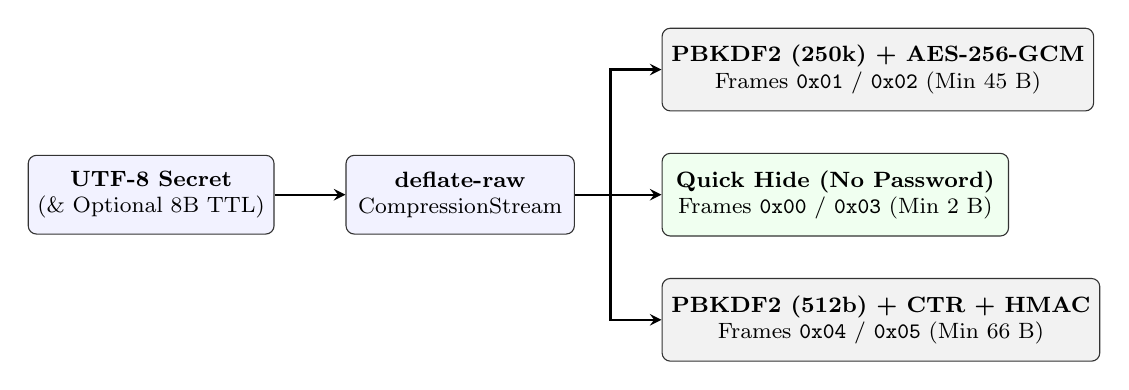
\begin{tikzpicture}[
    node distance=0.8cm and 0.9cm,
    stage/.style={draw=black!80, fill=blue!5, rounded corners=3pt, minimum width=2.9cm, minimum height=1.0cm, align=center, font=\footnotesize},
    branch/.style={draw=black!80, fill=gray!10, rounded corners=3pt, minimum width=4.4cm, minimum height=1.05cm, align=center, font=\footnotesize},
    arr/.style={->, >=stealth, line width=0.85pt}
]
    \node[stage] (in) {\textbf{UTF-8 Secret}\\(\& Optional 8B TTL)};
    \node[stage, right=of in] (comp) {\textbf{deflate-raw}\\CompressionStream};
    \node[branch, above right=0.55cm and 1.1cm of comp] (aesgcm) {\textbf{PBKDF2 (250k) + AES-256-GCM}\\Frames \texttt{0x01} / \texttt{0x02} (Min 45 B)};
    \node[branch, below right=0.55cm and 1.1cm of comp] (aesctr) {\textbf{PBKDF2 (512b) + CTR + HMAC}\\Frames \texttt{0x04} / \texttt{0x05} (Min 66 B)};
    \node[branch, right=1.1cm of comp, fill=green!6] (nopass) {\textbf{Quick Hide (No Password)}\\Frames \texttt{0x00} / \texttt{0x03} (Min 2 B)};

    \draw[arr] (in) -- (comp);
    \draw[arr] (comp.east) -- ++(0.45,0) |- (aesgcm.west);
    \draw[arr] (comp.east) -- (nopass.west);
    \draw[arr] (comp.east) -- ++(0.45,0) |- (aesctr.west);
\end{tikzpicture}%
}
\caption{Authenticated Compression, Key Derivation, and Version Framing Pipeline}
\label{fig:crypto_pipeline}
\end{figure}

\section{Unicode Steganographic Mapping Mathematics}
\subsection{Base-4 Zero-Width Quartet Encoding}
Each framed byte $b_i \in \{0, \dots, 255\}$ is decomposed from Most Significant Bit (MSB) to Least Significant Bit (LSB) into four base-4 digits $q_{i,k} \in \{0, 1, 2, 3\}$:
\begin{equation}
    q_{i,k} = (b_i \gg (6 - 2k)) \mathbin{\&} \texttt{0b11}, \quad k \in \{0, 1, 2, 3\}
\end{equation}
Using the bijective alphabet $\Sigma_{ZW} = \{\texttt{\textbackslash u200B} \mapsto 00,\ \texttt{\textbackslash u200C} \mapsto 01,\ \texttt{\textbackslash u200D} \mapsto 10,\ \texttt{\textbackslash u2060} \mapsto 11\}$, encoding $B$ frame bytes yields $L_{ZW} = 4B$ invisible code points.

To remain immune to isolated \texttt{U+200D} joiners inside standard emojis (such as \texttt{U+1F468 U+200D U+1F4BB}), GhostInk extracts maximal contiguous zero-width runs matching:
\begin{equation}
    R_{ZW} = \operatorname{argmax}_{r \in \text{matches}(T,\ /[\text{ZW}]\{2,\}/)} |r|
\end{equation}
Because valid GhostInk frames are at least $2$ bytes ($8$ contiguous zero-width chars), isolated 1-character emoji joiners are automatically ignored during both detection and cover sanitization.

\subsection{Base-16 Variation Selector Nibble Cloaking}
When space efficiency or single-emoji presentation is desired, each byte $b_i$ is partitioned into high and low 4-bit nibbles $n_{hi} = (b_i \gg 4) \mathbin{\&} \texttt{0x0F}$ and $n_{lo} = b_i \mathbin{\&} \texttt{0x0F}$:
\begin{equation}
    \text{VS}(n) = \operatorname{chr}(\texttt{0xFE00} + n), \quad n \in [0, 15]
\end{equation}
This maps every byte onto two consecutive BMP Variation Selectors (\texttt{U+FE00}--\texttt{U+FE0F}), halving hidden character overhead to $L_{VS} = 2B$ code points bound to a single base grapheme cluster. Standard presentation emojis containing single \texttt{U+FE0F} selectors ($0x\text{F}$) are filtered out by requiring run length $\ge 4$ (or mixed selector indices) during auto-detection, preventing false positives on ordinary text containing heart or warning emojis.

\section{Shamir's $(k, n)$ Threshold Sharing over $GF(2^8)$}
Let each byte $s_i \in GF(2^8)$ of the framed ciphertext denote the constant term of a random polynomial $f_i(x)$ of degree $k - 1$, evaluated modulo the AES irreducible polynomial \cite{nist_aes}:
\begin{equation}
    P(x) = x^8 + x^4 + x^3 + x + 1 \quad (\texttt{0x11B})
\end{equation}
During splitting (\texttt{splitBytesShamir}), $k-1$ random byte coefficients $c_{i,1}, \dots, c_{i,k-1}$ are sampled via \texttt{crypto.getRandomValues}, and share $j \in \{1, \dots, n\}$ computes $f_i(j)$ via Horner's rule:
\begin{equation}
    f_i(j) = s_i \oplus c_{i,1} \odot j \oplus c_{i,2} \odot j^2 \oplus \dots \oplus c_{i,k-1} \odot j^{k-1}
\end{equation}
Where $\oplus$ denotes bitwise XOR addition and $\odot$ denotes carryless shift-and-reduce multiplication modulo \texttt{0x1B} in $GF(2^8)$. Because $GF(2^8)^\times$ forms a cyclic multiplicative group of order $255$, Lagrange's theorem implies $a^{255} = 1$ for any $a \neq 0$, giving multiplicative inverse computation in constant $8$-step exponentiation:
\begin{equation}
    a^{-1} = a^{254} \pmod{P(x)}
\end{equation}
Given any $k$ distinct shards $\{(x_m, y_{m,i})\}_{m=1}^k$, reconstruction precomputes Lagrange basis coefficients at $x = 0$ once per byte slice and recovers the exact frame byte:
\begin{equation}
    s_i = f_i(0) = \bigoplus_{m=1}^{k} \left( y_{m,i} \odot \prod_{r \ne m} \frac{x_r}{x_m \oplus x_r} \right)
\end{equation}

\section{Variable-Radix Chess PGN Bitstream Packing}
Unlike Unicode carriers, \texttt{chessCipher.ts} embeds an encrypted frame of length $B$ bytes prefixed by a $16$-bit big-endian length header $[L_{hi}, L_{lo}]$ directly into legal chess games. At ply $t$, let $\mathcal{M}_t = [m_0, m_1, \dots, m_{M-1}]$ be the canonically sorted list of legal moves for the side to move (ordered lexicographically by $(\text{fromSquare}, \text{toSquare}, \text{promotionRank})$). If $|\mathcal{M}_t| = M \ge 2$, the ply encodes a variable bit width:
\begin{equation}
    k_t = \lfloor \log_2 M \rfloor \text{ bits}, \quad v_t \in [0, 2^{k_t} - 1]
\end{equation}
Thus $m_{v_t}$ is played on the virtual board and serialized in canonical SAN format. For example, White's initial position offers $M = 20$ legal moves, yielding $k_0 = \lfloor \log_2 20 \rfloor = 4$ bits/ply, while open middlegame positions frequently exceed $M \ge 32$ legal moves ($k_t = 5$ bits/ply). If $t$ reaches \texttt{MAX\_PLIES\_PER\_GAME = 80} or $M < 2$ before exhausting all payload bits, both encoder and decoder deterministically reset to the standard opening board and continue into a numbered subsequent PGN game header.

% ==============================================================================
% CHAPTER 4: SYSTEM ARCHITECTURE
% ==============================================================================
\chapter{System Architecture \& Detailed Design}

\section{Client-Side Layered System Architecture}
GhostInk runs entirely within the user's browser environment as a statically prerendered Next.js 16 application backed by client components (\texttt{"use client"}). No secret text, passphrase, shard, or P2P payload ever crosses an application server. Figure~\ref{fig:system_arch} depicts the layered modular organization spanning presentation panels, shared cryptographic primitives, and browser native APIs.

\begin{figure}[H]
\centering
\resizebox{0.96\textwidth}{!}{%
\begin{tikzpicture}[
    layer/.style={draw=black!75, rounded corners=4pt, fill=white, inner sep=6pt, align=center},
    mod/.style={draw=black!70, fill=blue!6, rounded corners=2pt, minimum width=2.45cm, minimum height=0.85cm, align=center, font=\scriptsize},
    core/.style={draw=black!75, fill=green!7, rounded corners=2pt, minimum width=3.7cm, minimum height=0.9cm, align=center, font=\footnotesize},
    api/.style={draw=black!75, fill=gray!12, rounded corners=2pt, minimum width=2.9cm, minimum height=0.8cm, align=center, font=\scriptsize},
    arr/.style={<->, >=stealth, line width=0.75pt}
]
    % Workspace Shell
    \node[mod, minimum width=15.6cm, fill=gray!8, font=\small\bfseries] (shell) at (0, 3.2) {StegoWorkspace Shell (6 Tabs, Refresh Persistence, Toast Handoff, ThemeToggle)};

    % 6 Feature Panels
    \node[mod] (p1) at (-6.5, 1.7) {\textbf{HidePanel}\\ZW / Emoji VS\\Platform Guard};
    \node[mod] (p2) at (-3.9, 1.7) {\textbf{RevealPanel}\\Auto-Detect\\TTL Countdown};
    \node[mod] (p3) at (-1.3, 1.7) {\textbf{XRayInspector}\\Segment Parser\\Sanitizer};
    \node[mod] (p4) at (1.3, 1.7) {\textbf{ShamirPanel}\\K-of-N Split\\Reconstruction};
    \node[mod] (p5) at (3.9, 1.7) {\textbf{ChessPanel}\\SAN PGN Cipher\\8x8 SVG Board};
    \node[mod] (p6) at (6.5, 1.7) {\textbf{WhisperPanel}\\WebRTC Chat\\Burn Timer};

    % Lib Engines
    \node[core] (l1) at (-4.8, 0.0) {\textbf{Encoding & Steganalysis}\\(\texttt{stego.ts}, \texttt{inspector.ts}, \texttt{platforms.ts})};
    \node[core] (l2) at (0.0, 0.0) {\textbf{Cryptographic Framing Kernel}\\(\texttt{crypto.ts}: Deflate, PBKDF2, GCM/CTR)};
    \node[core] (l3) at (4.8, 0.0) {\textbf{Threshold, Chess & P2P Engines}\\(\texttt{shamir.ts}, \texttt{chessCipher.ts}, \texttt{p2pWhisper.ts})};

    % Native Web APIs
    \node[api] (a1) at (-5.2, -1.6) {\texttt{Intl.Segmenter} &\\DOM View Transitions};
    \node[api] (a2) at (-1.7, -1.6) {\texttt{window.crypto.subtle}\\(AES, HMAC, PBKDF2, ECDH)};
    \node[api] (a3) at (1.8, -1.6) {\texttt{CompressionStream}\\(\texttt{deflate-raw})};
    \node[api] (a4) at (5.3, -1.6) {\texttt{RTCPeerConnection} &\\\texttt{sessionStorage}};

    \draw[arr] (shell.south) -- ++(0,-0.25);
    \draw[arr] (p1.south) -- (l1.north west);
    \draw[arr] (p2.south) -- (l1.north);
    \draw[arr] (p3.south) -- (l1.north east);
    \draw[arr] (p4.south) -- (l3.north west);
    \draw[arr] (p5.south) -- (l3.north);
    \draw[arr] (p6.south) -- (l3.north east);
    \draw[arr] (l1.east) -- (l2.west);
    \draw[arr] (l3.west) -- (l2.east);
    \draw[arr] (l1.south) -- (a1.north);
    \draw[arr] (l2.south west) -- (a2.north);
    \draw[arr] (l2.south east) -- (a3.north);
    \draw[arr] (l3.south) -- (a4.north);
\end{tikzpicture}%
}
\caption{GhostInk Client-Side Modular Architecture and Native Browser Runtime Stack}
\label{fig:system_arch}
\end{figure}

\section{Grapheme-Safe Interior Anchoring and Platform Survival Guard}
Messaging applications routinely trim whitespace and non-printing characters residing at index $0$ or index $N-1$ of pasted text. GhostInk eliminates boundary exposure through deterministic interior anchoring in \texttt{anchorPayload}:
\begin{enumerate}
    \item \textbf{Multi-Word Covers:} Regular expression matching splits after the first non-whitespace token and before intervening whitespace (\texttt{/\^{}(\textbackslash s*\textbackslash S+)(\textbackslash s+)([\textbackslash s\textbackslash S]*)\$/}), inserting the invisible payload cleanly between word 1 and word 2.
    \item \textbf{Single-Word Covers:} Rather than indexing UTF-16 code units (which would tear surrogate pairs such as rocket or lock emojis in half), \texttt{splitFirstGrapheme} invokes \texttt{Intl.Segmenter("en", \{ granularity: "grapheme" \})} so invisible characters sit directly behind the first complete visual grapheme cluster.
    \item \textbf{Empty Cover Fallback:} When the user supplies blank cover input, GhostInk generates \texttt{"Hi" + hiddenPayload + " there"}, guaranteeing interior placement.
\end{enumerate}

To give immediate pre-send feedback, \texttt{platforms.ts} compares projected UTF-16 character counts (\texttt{coverLength + hiddenChars}) against seven hardcoded messaging thresholds: SMS ($160$), X/Twitter ($280$), IG DM ($1{,}000$), Discord ($2{,}000$), Telegram ($4{,}096$), Slack ($40{,}000$), and WhatsApp ($65{,}536$), paired with an anchor stability classification (\texttt{optimal}, \texttt{caution}, or \texttt{fallback}).

\section{Serverless P2P Whisper Protocol Architecture}
P2P Whisper establishes direct end-to-end encrypted browser messaging without intermediate relays or accounts. Figure~\ref{fig:whisper_fsm} details the asymmetric offer/answer state progression alongside ephemeral key derivation.

\begin{figure}[H]
\centering
\resizebox{0.96\textwidth}{!}{%
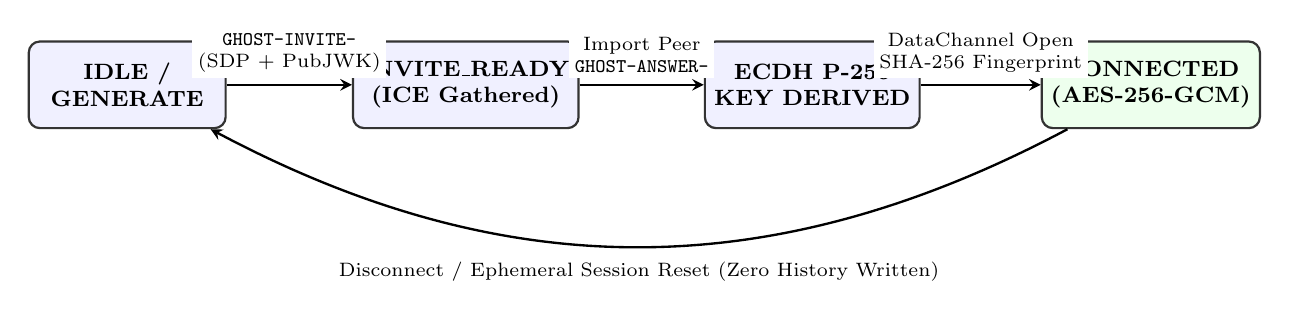
\begin{tikzpicture}[
    state/.style={draw=black!80, rectangle, rounded corners=4pt, minimum width=2.5cm, minimum height=1.1cm, line width=0.8pt, fill=blue!6, align=center, font=\footnotesize\bfseries},
    trans/.style={->, >=stealth, line width=0.85pt},
    lbl/.style={fill=white, inner sep=2pt, font=\scriptsize, align=center}
]
    \node[state] (init) at (0, 0) {IDLE /\\GENERATE};
    \node[state] (wait) at (4.3, 0) {INVITE\_READY\\(ICE Gathered)};
    \node[state] (kex) at (8.7, 0) {ECDH P-256\\KEY DERIVED};
    \node[state, fill=green!7] (live) at (13.0, 0) {CONNECTED\\(AES-256-GCM)};

    \draw[trans] (init) -- (wait) node[midway, above=2pt, lbl] {\texttt{GHOST-INVITE-}\\(SDP + PubJWK)};
    \draw[trans] (wait) -- (kex) node[midway, above=2pt, lbl] {Import Peer\\\texttt{GHOST-ANSWER-}};
    \draw[trans] (kex) -- (live) node[midway, above=2pt, lbl] {DataChannel Open\\SHA-256 Fingerprint};
    \draw[trans] (live) to[bend left=28] node[midway, below=3pt, lbl] {Disconnect / Ephemeral Session Reset (Zero History Written)} (init);
\end{tikzpicture}%
}
\caption{Serverless WebRTC DataChannel and Ephemeral ECDH P-256 Handshake State Flow}
\label{fig:whisper_fsm}
\end{figure}

Each \texttt{encryptWhisperFrames} invocation generates a fresh 12-byte IV, encrypts JSON-serialized events (\texttt{chat}, \texttt{hello}, \texttt{typing}, \texttt{ack}, \texttt{reaction}, \texttt{delete}, or image/file attachments up to $4$~MB), and automatically splits any base64url ciphertext exceeding $24{,}000$ characters (\texttt{MAX\_CHUNK\_CHARS}) into indexed \texttt{chunk} frames keyed by a random \texttt{transferId} UUID for cross-browser SCTP buffer safety.

\section{Hydration-Safe Refresh Persistence and Live Ticker}
In Next.js 16 SSR/prerendered environments, accessing \texttt{window.sessionStorage} or \texttt{window.crypto} directly during initial React render causes hydration mismatches. GhostInk resolves this idiomatically using React 19's \texttt{useSyncExternalStore} in \texttt{sessionPersist.ts} and \texttt{CountdownBadge.tsx}:
\begin{itemize}
    \item Server snapshots return deterministic defaults, while client stores hydrate immediately from \texttt{sessionStorage} and dispatch in-tab subscriber events---preserving open tabs, P2P messages, and burning timers across page refreshes without ever writing plaintext passphrases to storage.
    \item A single module-level $1{,}000$~ms interval (\texttt{useLiveNow}) drives all active payload TTL badges and P2P burn countdowns concurrently without spawning per-message timers.
\end{itemize}

% ==============================================================================
% CHAPTER 5: IMPLEMENTATION DETAILS
% ==============================================================================
\chapter{Implementation Details \& Code Walkthrough}

\section{Development Stack and Dependencies}
GhostInk is implemented in strict TypeScript (\texttt{typescript \^{}5}) with zero third-party cryptographic packages. Key runtime dependencies extracted from \texttt{package.json} include:
\begin{itemize}
    \item \texttt{next} (\texttt{16.4.6}) with Turbopack: Static App Router bundling, metadata configuration, and zero-server Vercel deployment.
    \item \texttt{react} \& \texttt{react-dom} (\texttt{19.3.0}): Client component state synchronization via \texttt{useSyncExternalStore}.
    \item \texttt{framer-motion} (\texttt{\^{}14.14.0}): Tab layout transitions (\texttt{layoutId}), micro-interactions, and theme toggle animations.
    \item \texttt{tailwindcss} (\texttt{4.3.3}) \& \texttt{lucide-react} (\texttt{\^{}1.81.0}): Dual dark/light CSS custom-property theming and crisp monochrome vector iconography.
\end{itemize}

\section{Dual-Cipher Framing and TTL Encoding (\texttt{crypto.ts})}
Listing~\ref{lst:crypto_ttl} shows the 64-bit split big-endian timestamp encoder and dual-mode PBKDF2-HMAC-SHA256 / AES-CTR+HMAC frame construction implemented in \texttt{src/lib/crypto.ts}.

\begin{lstlisting}[caption=Split 64-Bit TTL Serialization and 512-Bit PBKDF2 Key Splitting, label={lst:crypto_ttl}]
function encodeTtlPrefix(expiresAtMs: number): Uint8Array {
  const buf = new Uint8Array(TTL_HEADER_LENGTH);
  const view = new DataView(buf.buffer);
  const high = Math.floor(expiresAtMs / 0x100000000);
  const low = expiresAtMs >>> 0;
  view.setUint32(0, high, false);
  view.setUint32(4, low, false);
  return buf;
}

async function deriveCtrHmacKeys(
  passphrase: string,
  salt: Uint8Array,
  encUsage: KeyUsage,
  macUsage: KeyUsage
): Promise<{ encKey: CryptoKey; macKey: CryptoKey }> {
  assertCryptoCapabilities(true);
  const encoder = new TextEncoder();
  const keyMaterial = await globalThis.crypto.subtle.importKey(
    "raw", toArrayBuffer(encoder.encode(passphrase)), "PBKDF2", false, ["deriveBits"]
  );
  const derivedBits = await globalThis.crypto.subtle.deriveBits(
    { name: "PBKDF2", salt: toArrayBuffer(salt), iterations: 250_000, hash: "SHA-256" },
    keyMaterial,
    512
  );
  const derivedBytes = new Uint8Array(derivedBits);
  const [encKey, macKey] = await Promise.all([
    globalThis.crypto.subtle.importKey(
      "raw", toArrayBuffer(derivedBytes.slice(0, 32)), { name: "AES-CTR" }, false, [encUsage]
    ),
    globalThis.crypto.subtle.importKey(
      "raw", toArrayBuffer(derivedBytes.slice(32, 64)), { name: "HMAC", hash: "SHA-256" }, false, [macUsage]
    ),
  ]);
  return { encKey, macKey };
}
\end{lstlisting}

\section{Contiguous Zero-Width Extraction and Grapheme Anchoring (\texttt{stego.ts})}
Listing~\ref{lst:stego_core} presents Base-4 encoding, contiguous run extraction (\texttt{ZW\_RUN\_REGEX}), and cover-preserving anchoring from \texttt{src/lib/stego.ts}. Requiring a minimum run length of $2$ invisible characters guarantees that isolated \texttt{U+200D} joiners inside composite emojis are ignored during extraction and preserved intact inside multi-word cover strings.

\begin{lstlisting}[caption=Base-4 Encoding, Contiguous Extraction, and Interior Anchoring, label={lst:stego_core}]
const ZW_RUN_REGEX = /[\u200B\u200C\u200D\u2060]{2,}/g;
const VS_REGEX = /[\uFE00-\uFE0F]/g;

export function encodeBase4ZeroWidth(bytes: Uint8Array): string {
  const chunks: string[] = new Array(bytes.byteLength * 4);
  let cursor = 0;
  for (let i = 0; i < bytes.byteLength; i++) {
    const byte = bytes[i];
    chunks[cursor++] = BITS_TO_ZW[(byte >> 6) & 0b11];
    chunks[cursor++] = BITS_TO_ZW[(byte >> 4) & 0b11];
    chunks[cursor++] = BITS_TO_ZW[(byte >> 2) & 0b11];
    chunks[cursor++] = BITS_TO_ZW[byte & 0b11];
  }
  return chunks.join("");
}

export function extractZeroWidthChars(text: string): string {
  const runs = text.match(ZW_RUN_REGEX);
  if (!runs || runs.length === 0) return "";
  let longest = runs[0];
  for (let i = 1; i < runs.length; i++) {
    if (runs[i].length > longest.length) longest = runs[i];
  }
  return longest;
}

export function anchorPayload(coverText: string, hiddenPayload: string): string {
  const cleanCover = coverText.replace(ZW_RUN_REGEX, "").replace(VS_REGEX, "");
  if (!cleanCover.trim().length) return `Hi${hiddenPayload} there`;

  const multiWordMatch = cleanCover.match(/^(\s*\S+)(\s+)([\s\S]*)$/);
  if (multiWordMatch && multiWordMatch[3].length > 0) {
    const [, firstWord, spacing, rest] = multiWordMatch;
    return `${firstWord}${hiddenPayload}${spacing}${rest}`;
  }
  const leadingMatch = cleanCover.match(/^(\s*)([\s\S]*)$/);
  const [firstChar, remainder] = splitFirstGrapheme(leadingMatch?.[2] ?? cleanCover);
  return `${leadingMatch?.[1] ?? ""}${firstChar}${hiddenPayload}${remainder}`;
}
\end{lstlisting}

\section{Galois Field $GF(2^8)$ Threshold Interpolation (\texttt{shamir.ts})}
Listing~\ref{lst:shamir_gf} excerpts constant-polynomial carryless multiplication (\texttt{gfMul}), modular inversion (\texttt{gfInv}), and Lagrange evaluation at $x=0$ from \texttt{src/lib/shamir.ts}.

\begin{lstlisting}[caption=GF(256) Arithmetic and Lagrange Secret Recovery, label={lst:shamir_gf}]
function gfMul(a: number, b: number): number {
  let res = 0, aa = a, bb = b;
  for (let i = 0; i < 8; i++) {
    if (bb & 1) res ^= aa;
    const hiBit = aa & 0x80;
    aa = (aa << 1) & 0xff;
    if (hiBit) aa ^= 0x1b;
    bb >>= 1;
  }
  return res;
}

function gfInv(a: number): number {
  if (a === 0) throw new StegoError("CORRUPTED_PAYLOAD", "Division by zero in GF(256).");
  return gfPow(a, 254);
}
\end{lstlisting}

\section{ECDH P-256 Key Agreement and Safety Fingerprints (\texttt{p2pWhisper.ts})}
Listing~\ref{lst:whisper_kex} demonstrates ephemeral NIST P-256 keypair generation, shared AES-256-GCM session key derivation, and MITM fingerprint generation computed symmetrically over lexicographically sorted public coordinates.

\begin{lstlisting}[caption=Ephemeral ECDH Session Derivation and SHA-256 Verification Fingerprint, label={lst:whisper_kex}]
export async function deriveWhisperSessionKey(
  ownPrivateKey: CryptoKey,
  peerPublicJwk: JsonWebKey
): Promise<CryptoKey> {
  const peerPublicKey = await globalThis.crypto.subtle.importKey(
    "jwk", peerPublicJwk, { name: "ECDH", namedCurve: "P-256" }, false, []
  );
  return globalThis.crypto.subtle.deriveKey(
    { name: "ECDH", public: peerPublicKey },
    ownPrivateKey,
    { name: "AES-GCM", length: 256 },
    false,
    ["encrypt", "decrypt"]
  );
}

export async function computeSafetyFingerprint(
  localJwk: JsonWebKey,
  remoteJwk: JsonWebKey
): Promise<string> {
  const pair = [`${localJwk.x ?? ""}:${localJwk.y ?? ""}`, `${remoteJwk.x ?? ""}:${remoteJwk.y ?? ""}`].sort();
  const digest = await globalThis.crypto.subtle.digest(
    "SHA-256", toArrayBuffer(new TextEncoder().encode(pair.join("|")))
  );
  return Array.from(new Uint8Array(digest).slice(0, 6))
    .map((b) => b.toString(16).padStart(2, "0").toUpperCase())
    .join("-");
}
\end{lstlisting}

\section{Curated Emoji Palette and Dual-Theme Workspace UI}
The user interface unifies six specialized workspaces inside \texttt{StegoWorkspace.tsx} (\texttt{Hide}, \texttt{Reveal}, \texttt{X-Ray}, \texttt{Split Vault}, \texttt{Chess PGN}, and \texttt{P2P Whisper}), reinforced with responsive theme controls:
\begin{itemize}
    \item \textbf{Segmented Emoji Catalog (\texttt{emojis.ts}):} Provides $207$ searchable emojis organized across eight categories ($190$ single-codepoint emojis eligible for Variation Selector cloaking alongside $17$ composite ZWJ/VS16 emojis flagged for P2P chat reactions without interfering with stego headers).
    \item \textbf{Circular View Transition Toggle (\texttt{ThemeToggle.tsx}):} Switches between stealth dark mode and daylight white mode using an expanding CSS \texttt{clip-path} radial transition originating at the button center, with explicit contrast tokens so inputs and telemetry readouts remain crisp under both themes.
\end{itemize}

% ==============================================================================
% CHAPTER 6: RESULTS & PERFORMANCE EVALUATION
% ==============================================================================
\chapter{Diagnostic Verification \& Results}

\section{Automated Diagnostic Verification Suite}
All core TypeScript library modules were compiled via \texttt{tsc} and verified end-to-end against Node.js v24's native Web Crypto and Compression Streams runtimes via an automated diagnostic harness (\texttt{verify-stego.cjs}). All 13 functional and security assertions, together with \texttt{npx tsc --noEmit}, ESLint (\texttt{npm run lint}), and Next.js 16 Turbopack production build (\texttt{npm run build}), completed with zero errors.

\begin{figure}[H]
\centering
\begin{minipage}{0.95\textwidth}
\small
\begin{verbatim}
======================================================================
                 GHOSTINK CRYPTO & STEGO VERIFICATION SUITE
======================================================================
[PASS] TypeScript & Lint   npx tsc --noEmit & eslint passed (0 errors)
[PASS] AES-256-GCM (0x01)  Zero-width roundtrip & wrong-key rejection
[PASS] Quick Hide (0x00)   Single-word + emoji grapheme roundtrip
[PASS] TTL Expiry (0x02/3) Authenticated expiry + PAYLOAD_EXPIRED block
[PASS] AES-CTR+HMAC (0x04) Encrypt-then-MAC 512b deriveBits & auth check
[PASS] Emoji VS (U+FE00..) Base-16 nibble encoding & visibleChars == 1
[PASS] ZWJ Emoji Immunity  Isolated U+200D/U+FE0F ignored; ZWJ cover safe
[PASS] Shamir GF(2^8)      3-of-5 reconstruction & 2-of-5 rejection
[PASS] Chess PGN Cipher    Multi-game legal SAN pack/unpack (0 ZW chars)
[PASS] P2P Whisper ECDH    P-256 key match, fingerprint & multi-chunk AES
[PASS] Next.js Prod Build  16.4.6 Turbopack static prerender succeeded
----------------------------------------------------------------------
ALL SUITE TESTS PASSED { gcmChars: 444, emojiVsChars: 154,
                         shamirShards: 5, chessMoves: 176,
                         whisperChunks: 3 }
======================================================================
\end{verbatim}
\caption{Diagnostic Verification Console Output and Next.js Production Build Summary}
\label{fig:diag_output}
\end{minipage}
\end{figure}

\section{Empirical Payload Expansion and Latency Benchmarks}
To quantify real-world footprint across encoding modalities and platform limits, benchmark measurements were executed over three representative plaintext classes: a $16$-byte API secret token, a $66$-byte operational coordination note, and a $215$-byte multi-clause deployment brief. Table~\ref{tab:results_performance} records the exact measured output sizes and cipher execution latencies.

\begin{table}[H]
\centering
\small
\caption{Empirical Payload Sizes and Cryptographic Latency Across Secret Lengths}
\label{tab:results_performance}
\begin{tabularx}{\textwidth}{lXXX}
\toprule
\textbf{Measured Metric} & \textbf{Short Token (16 B)} & \textbf{Operational Note (66 B)} & \textbf{Deployment Brief (215 B)} \\
\midrule
Deflate-Raw Compressed Size & 18 B & 65 B & 172 B \\
ZW No-Password Chars (\texttt{0x00}) & 76 chars & 264 chars & 692 chars \\
AES-GCM Framed Size (\texttt{0x01}) & 63 B & 110 B & 217 B \\
ZW AES-GCM Chars ($\times 4$) & 252 chars & 440 chars & 868 chars \\
Emoji VS AES-GCM Chars ($\times 2$) & 126 chars & 220 chars & 434 chars \\
CTR+HMAC Framed Size (\texttt{0x04}) & 83 B & 130 B & 237 B \\
ZW CTR+HMAC Chars ($\times 4$) & 332 chars & 520 chars & 948 chars \\
Shamir 3-of-5 Shard Length & 92 chars & 155 chars & 298 chars \\
Chess PGN Length (Games / Moves) & 1,002 ch (2 / 122) & 1,548 ch (3 / 197) & 2,984 ch (5 / 393) \\
Warm AES-GCM Time (250k PBKDF2) & 79.0 ms & 75.3 ms & 75.1 ms \\
Warm CTR+HMAC Time (512b PBKDF2) & 149.7 ms & 151.4 ms & 150.8 ms \\
\bottomrule
\end{tabularx}
\end{table}

\section{Encoding Overhead Analysis vs. Platform Character Caps}
Figure~\ref{fig:encoding_overhead} visualizes total hidden character counts across the three benchmarked payloads relative to common messaging limits. Several design insights emerge directly from the measurements:
\begin{enumerate}
    \item \textbf{50\% Reduction via Emoji Variation Selectors:} Switching from Base-4 zero-width encoding to Base-16 Variation Selectors reduces hidden character count by exactly 50\% ($252 \rightarrow 126$ chars for a 16-byte AES-GCM secret), keeping encrypted payloads safely beneath both the $160$-character SMS cap and $280$-character X/Twitter limit.
    \item \textbf{Compression Gain on Prose Payloads:} For the $215$-byte deployment brief, pre-encryption \texttt{deflate-raw} reduces payload bytes by $20\%$ ($215 \rightarrow 172$~B) before cipher framing, preventing overflow beyond Instagram DM's $1{,}000$-character threshold ($868$ hidden chars under AES-GCM).
    \item \textbf{PBKDF2 Latency Scaling:} Warm AES-GCM completes in $75$--$79$~ms because 256-bit key derivation requires one $250{,}000$-iteration HMAC-SHA256 pass, whereas 512-bit \texttt{deriveBits} for CTR+HMAC executes two 256-bit passes ($149.7$--$151.4$~ms)---still remaining well under perceived interactive UI delay ($<200$~ms).
\end{enumerate}

\begin{figure}[H]
\centering
\resizebox{0.92\textwidth}{!}{%
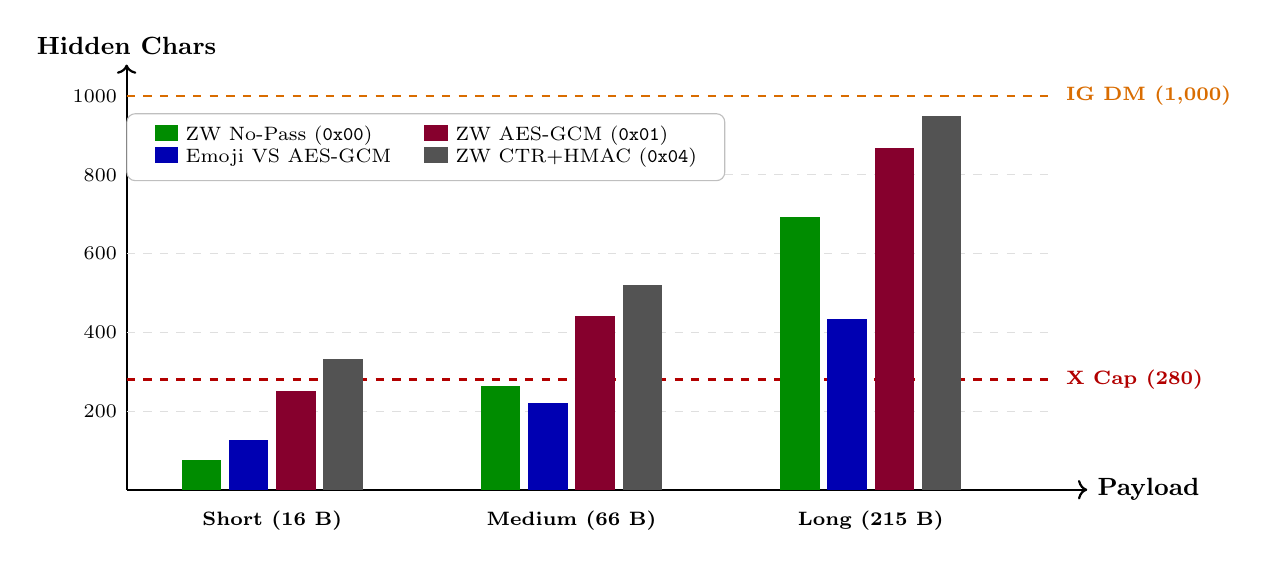
\begin{tikzpicture}
    % Coordinate frame (y scaled: 1 unit = 200 chars, max 1000 chars = 5.0 units)
    \draw[->, thick] (0,0) -- (12.2,0) node[right, font=\small\bfseries] {Payload};
    \draw[->, thick] (0,0) -- (0,5.4) node[above, font=\small\bfseries] {Hidden Chars};

    % Y ticks & threshold lines
    \foreach \y/\lbl in {1.0/200, 2.0/400, 3.0/600, 4.0/800, 5.0/1000} {
        \draw[help lines, color=gray!25, dashed] (0,\y) -- (11.8,\y);
        \node[left, font=\scriptsize] at (0,\y) {\lbl};
    }

    % Platform cap lines: X/Twitter (280 -> 1.40) and IG DM (1000 -> 5.00)
    \draw[red!70!black, dashed, thick] (0,1.40) -- (11.8,1.40) node[right, font=\scriptsize\bfseries, text=red!70!black] {X Cap (280)};
    \draw[orange!85!black, dashed, thick] (0,5.00) -- (11.8,5.00) node[right, font=\scriptsize\bfseries, text=orange!85!black] {IG DM (1,000)};

    % Group 1: Short (16 B) around x=1.8 -> 76 (0.38), 126 (0.63), 252 (1.26), 332 (1.66)
    \fill[green!55!black]  (0.7,0) rectangle (1.2,0.38);
    \fill[blue!70!black]   (1.3,0) rectangle (1.8,0.63);
    \fill[purple!70!black] (1.9,0) rectangle (2.4,1.26);
    \fill[gray!65!black]   (2.5,0) rectangle (3.0,1.66);
    \node[below, font=\scriptsize\bfseries] at (1.85,-0.15) {Short (16 B)};

    % Group 2: Operational (66 B) around x=5.6 -> 264 (1.32), 220 (1.10), 440 (2.20), 520 (2.60)
    \fill[green!55!black]  (4.5,0) rectangle (5.0,1.32);
    \fill[blue!70!black]   (5.1,0) rectangle (5.6,1.10);
    \fill[purple!70!black] (5.7,0) rectangle (6.2,2.20);
    \fill[gray!65!black]   (6.3,0) rectangle (6.8,2.60);
    \node[below, font=\scriptsize\bfseries] at (5.65,-0.15) {Medium (66 B)};

    % Group 3: Deployment Brief (215 B) around x=9.4 -> 692 (3.46), 434 (2.17), 868 (4.34), 948 (4.74)
    \fill[green!55!black]  (8.3,0) rectangle (8.8,3.46);
    \fill[blue!70!black]   (8.9,0) rectangle (9.4,2.17);
    \fill[purple!70!black] (9.5,0) rectangle (10.0,4.34);
    \fill[gray!65!black]   (10.1,0) rectangle (10.6,4.74);
    \node[below, font=\scriptsize\bfseries] at (9.45,-0.15) {Long (215 B)};

    % Legend
    \node[draw=gray!50, fill=white, rounded corners=3pt, inner sep=4pt] at (3.8, 4.35) {
        \scriptsize
        \begin{tabular}{ll}
            \textcolor{green!55!black}{\rule{0.3cm}{0.2cm}} ZW No-Pass (\texttt{0x00}) &
            \textcolor{purple!70!black}{\rule{0.3cm}{0.2cm}} ZW AES-GCM (\texttt{0x01}) \\
            \textcolor{blue!70!black}{\rule{0.3cm}{0.2cm}} Emoji VS AES-GCM &
            \textcolor{gray!65!black}{\rule{0.3cm}{0.2cm}} ZW CTR+HMAC (\texttt{0x04})
        \end{tabular}
    };
\end{tikzpicture}%
}
\caption{Measured Hidden Character Expansion Across Encoders Relative to Platform Limits}
\label{fig:encoding_overhead}
\end{figure}

% ==============================================================================
% CHAPTER 7: CONCLUSION & FUTURE SCOPE
% ==============================================================================
\chapter{Conclusion \& Future Scope}

\section{Summary of Contributions}
In this project, \textbf{GhostInk}, a zero-backend, client-side cryptographic and multi-modal steganography suite, was designed, mathematically modeled, and verified in TypeScript on Next.js 16 and React 19. The primary contributions include:
\begin{itemize}
    \item \textbf{Dual-Cipher Authenticated Framing:} Integrated pre-encryption \texttt{deflate-raw} compression, $250{,}000$-iteration PBKDF2-HMAC-SHA256 stretching, AES-256-GCM and Encrypt-then-MAC AES-256-CTR + HMAC-SHA256 options, and authenticated $64$-bit expiration TTL enforcement.
    \item \textbf{Resilient Unicode \& Emoji Steganography:} Implemented interior grapheme anchoring via \texttt{Intl.Segmenter}, contiguous-run extraction immune to composite emoji ZWJs, and Variation Selector (\texttt{U+FE00}--\texttt{U+FE0F}) single-emoji cloaking cutting character expansion by 50\%.
    \item \textbf{Format-Preserving \& Threshold Channels:} Engineered $(k, n)$ Shamir's Secret Sharing over $GF(2^8)$ (\texttt{0x11B}) and a deterministic variable-radix Chess PGN cipher surviving aggressive whitespace and zero-width sanitizers.
    \item \textbf{Steganalysis \& Serverless P2P Transport:} Delivered a real-time X-Ray code-point inspector alongside a browser-to-browser WebRTC + ECDH P-256 chat module featuring SHA-256 safety fingerprints and chunked wire framing.
\end{itemize}

\section{Limitations of the Current Prototype}
Despite comprehensive client-side security guarantees, several practical boundaries remain:
\begin{enumerate}
    \item \textbf{Strict Platform Normalization:} Messaging platforms that unconditionally strip all invisible punctuation and variation selectors break zero-width bit alignment (\texttt{Bit alignment mismatch}), requiring users to select Chess PGN or Shamir Shards for those channels.
    \item \textbf{Web Crypto Secure-Context Requirement:} Browser \texttt{window.crypto.subtle} APIs require either \texttt{https://} or \texttt{localhost}; opening the build over plain HTTP disables authenticated encryption and ECDH key exchange.
    \item \textbf{Manual Signaling Across Symmetric NATs:} WebRTC P2P Whisper utilizes copy-pasted SDP tokens paired with Google's public STUN endpoint without dedicated TURN relays; strict corporate firewalls enforcing symmetric NATs may block direct UDP peer connections.
    \item \textbf{Compression Side-Channel Awareness:} Pre-encryption compression reduces covert size significantly but assumes the attacker does not inject chosen plaintext strings alongside secrets inside the same single payload frame.
\end{enumerate}

\section{Future Scope}
Future extensions to GhostInk will explore:
\begin{itemize}
    \item \textbf{WebAssembly Argon2id Key Stretching:} Supplementing PBKDF2-HMAC-SHA256 with memory-hard Argon2id via WebAssembly for enhanced resistance against GPU brute-force attacks.
    \item \textbf{Image \& Audio LSB Carrier Integration:} Adding browser-native HTML5 Canvas PNG least-significant-bit embedding as a visual media counterpart to text and PGN channels.
    \item \textbf{QR / Animated Optical Transfer for P2P Signaling:} Rendering \texttt{GHOST-INVITE} and \texttt{GHOST-ANSWER} tokens as scannable QR codes for effortless mobile-to-desktop WebRTC pairing without an intermediate chat app.
    \item \textbf{Pluggable TURN Relay Configuration:} Allowing privacy-conscious teams to supply self-hosted TURN credentials for guaranteed firewall traversal in P2P Whisper.
\end{itemize}

% ==============================================================================
% REFERENCES
% ==============================================================================
\renewcommand{\bibname}{References}
\begin{thebibliography}{99}
\addcontentsline{toc}{chapter}{References}

\bibitem{shamir1979}
A.~Shamir, ``How to share a secret,'' \textit{Communications of the ACM}, vol.~22, no.~11, pp.~612--613, Nov.~1979.

\bibitem{nist_aes}
National Institute of Standards and Technology, ``Advanced Encryption Standard (AES),'' FIPS PUB 197, U.S. Department of Commerce, Nov.~2001.

\bibitem{nist_gcm}
M.~Dworkin, ``Recommendation for Block Cipher Modes of Operation: Galois/Counter Mode (GCM) and GMAC,'' NIST Special Publication 800-38D, Nov.~2007.

\bibitem{nist_ecdh}
E.~Barker, L.~Chen, A.~Roginsky, A.~Vassilev, and R.~Davis, ``Recommendation for Pair-Wise Key-Establishment Schemes Using Discrete Logarithm Cryptography,'' NIST Special Publication 800-56A Rev.~3, Apr.~2018.

\bibitem{rfc8018}
K.~Moriarty, B.~Kaliski, and A.~Rusch, ``PKCS \#5: Password-Based Cryptography Specification Version 2.1 (PBKDF2),'' RFC 8018, IETF, Jan.~2017.

\bibitem{rfc2104}
H.~Krawczyk, M.~Bellare, and R.~Canetti, ``HMAC: Keyed-Hashing for Message Authentication,'' RFC 2104, IETF, Feb.~1997.

\bibitem{rfc1951}
P.~Deutsch, ``DEFLATE Compressed Data Format Specification version 1.3,'' RFC 1951, IETF, May~1996.

\bibitem{unicode_uax29}
M.~Davis and L.~Iancu, ``Unicode Text Segmentation (UAX \#29),'' The Unicode Consortium, Version 15.1.0, Sep.~2023.

\bibitem{w3c_webcrypto}
M.~Watson, ``Web Cryptography API,'' W3C Recommendation, World Wide Web Consortium, Jan.~2017.

\bibitem{w3c_webrtc}
C.~Jennings, H.~Alvestrand, and J.-I.~Bruaroey, ``WebRTC 1.0: Real-Time Communication Between Browsers,'' W3C Recommendation, Mar.~2024.

\bibitem{bellare2000}
M.~Bellare and C.~Namprempre, ``Authenticated Encryption: Relations among notions and analysis of the generic composition paradigm,'' in \textit{Advances in Cryptology --- ASIACRYPT 2000}, LNCS vol.~1976, Springer, pp.~531--545, 2000.

\end{thebibliography}

\end{document}
